%!TEX root = main.tex

\chapter[Mitigating Initialisation Impact by Real-Time Control: Online PAC-Bayes Learning]{Mitigating Initialisation Impact by Real-Time Control: Online PAC-Bayes Learning}
\label{chap:online-pb}

\addchapterlof
\addchapterloa
\addchapterloe

\vspace{-1.0cm}
\begin{center}
\textbf{This chapter is based on the following papers}\\[0.1cm]
\end{center}
\printpublication{haddouche2022online}
\\
\printpublication{haddouche2023pac}


\vspace{0.2cm}
\minitoc

\begin{abstract}
  While \Cref{chap: pb-ht} showed weak statistical assumptions were reachable in PAC-Bayes, allowing its use in a wide range of concrete optimisation settings, the role of the prior $\P$ remains untreated. To tackle this issue, we propose here to consider $\P$ as the initialisation point of a learning algorithm. Then, to attenuate its impact in PAC-Bayes procedures, we develop \emph{Online PAC-Bayes learning}, which consider a sequence $(\Q_{i},\P_{i})_{i=1\cdots m}$ of pairs (posterior,prior) evolving through time. Thus, the impact of initialisation $\P=\P_1$ is attenuated through the evolution of $\P_{i}$ during the learning phase. We develop the first Online PAC-Bayes bounds and propose experiments showing that online PAC-Bayes outperforms SGD in several cases.
\end{abstract}


\section{Introduction}

 Batch learning is somewhat the dominant learning paradigm in which we aim to design the best predictor by collecting a training dataset which is then used for inference or prediction. Classical algorithms such as SVMs \citep[see][among many others]{cristianini2000introduction} or feedforward neural networks \citep{svozil1997introduction} are popular examples of efficient batch learning. While the mathematics of batch learning constitute a vivid and well understood research field, in practice this might not be aligned with the way practitionners collect data, which can be sequential when too much information is available at a given time (\emph{e.g.} the number of microtransactions made in finance on a daily basis). Indeed, batch learning is not designed to properly handle dynamic systems.


 Online learning (OL)  \citep{zinkevich2003online,shalev2012online,hazan2016introduction} fills this gap by treating data as a continuous stream with a potentially changing learning goal.
 OL has been studied with convex optimisation tools and the celebrated notion of regret which measures the discrepancy between the cumulative sum of losses for a specific algorithm at each datum and the optimal strategy. It led to many fruitful results comparing the  efficiency of prediction for optimisation algorithms such that Online Gradient Descent (OGD), Online Newton Step through static regret \citep{zinkevich2003online,hazan2007logarithmic}. OL is flexible enough to incorporate external expert advice onto classical algorithms with the optimistic point of view that such advices are useful for training \citep{rakhlin2013online,rakhlin2013practical} and then having optimistic regret bounds.
 Modern extensions also allow to compare to moving strategies through dynamic regret \citep[see e.g.][]{yang2016tracking,zhang2018strong,zhao2020dyn}. However, this notion of regret has been challenged recently: for instance, \citet{wintenberger2021stochastic} chose to control an expected cumulative loss through PAC inequalities in order to deal with the case of stochastic loss functions.

While OL tackles problems beyond batch learning, it can also be used as a tool to understand stochastic methods in a batch framework, such as SGD, where data are picked sequentially. In the context of PAC-Bayes, it is then natural to ask whether online learning could explain either the in-training evolution of the generalisation ability of batch methods or provide online variants of classical algorithms (\eg \eqref{eq: alg-mcall}, \eqref{eq: alg-catoni}). In both cases, the online paradigm allows focusing less on the prior $\P$ and more on its evolution, being consistent with the optimisation view of the prior as an initialisation point (see \Cref{fig: recap-optim}). 

\textbf{Our contributions.} Our goal is to provide a general online framework for PAC-Bayesian learning. Our main contribution (\Cref{th: main_thm_online} in \Cref{sec: main_bound}) is a general bound  valid for bounded losses exploiting the generic PAC-Bayes bound of \citet{rivasplata2020pac}, later used to derive several online PAC-Bayesian results (as developed in \Cref{sec: online_pacb_procedure,sec: OPBD_procedure}).
More specifically, we derive two types of bounds, \emph{online PAC-Bayesian training and test bounds}.
Training bounds exhibit online procedures while the test bound provide efficiency guarantees. We propose then several algorithms with their associated training and test bounds as well as a short series of experiments to evaluate the consistency of our online PAC-Bayesian approach. Our efficiency criterion is not the classical regret but an expected cumulative loss close to the one of \citet{wintenberger2021stochastic}. More precisely, \Cref{sec: online_pacb_procedure} propose a stable yet time-consuming Gibbs-based algorithm, while \Cref{sec: OPBD_procedure} proposes time efficient yet volatile algorithms.
However, even if OPB requires no assumption on the data distribution, allows priors to be data-dependent and do not require any convexity assumption on the loss (as commonly assumed in the OL framework), it still requires a bounded loss. We circumvent this limitation in \Cref{sec: heavy-tailed} that it is possible to extend OPB results to the case of heavy-tailed losses, exploiting the supermartingale toolbox of \Cref{chap: pb-ht}.

\textbf{Outline.} \Cref{sec: main_bound} introduces the  theoretical framework as well as our main result. \Cref{sec: online_pacb_procedure} presents an online PAC-Bayesian algorithm and draws links between PAC-Bayes and OL results.
\Cref{sec: OPBD_procedure} details online PAC-Bayesian disintegrated procedures with reduced computational time, \Cref{sec: experiments} gathers supporting experiments and \Cref{sec: heavy-tailed} gathers an extension of \Cref{sec: main_bound} for heavy-tailed losses.
We include reminders on OL and PAC-Bayes in \Cref{sec: OGD_reminder,sec: disintegrated_bounds}. \Cref{sec: discussion_main_thm} provide discussion about our main result. All proofs are deferred to \Cref{sec: proofs-chap3}.

\section{An online PAC-Bayesian bound for bounded losses}
\label{sec: main_bound}
We establish a novel PAC-Bayesian theorem (which in turn will be particularised in \Cref{sec: online_pacb_procedure}) overcoming the classical limitation of data-independent prior and \iid data.
We call our main result an \emph{online PAC-Bayesian bound} as it allows to consider a sequence of priors which may depend on the past and a sequence of posteriors that can dynamically evolve as well. Indeed, we follow the online learning paradigm which considers a continous stream of data that the algorithm has to process on the fly, adjusting its outputs at each time step \wrt the arrival of new data and the past. In the PAC-Bayesian framework, this paradigm translates as follows: from an initial (still data independent) prior $\Q_1=\P$ and a data sample $\Sm= (z_1,...,z_m)$, we design a sequence of posterior $(\Q_{i})_{1\leq i\leq m }$ where $\Q_{i}= f(\Q_1,...,\Q_{i-1},z_i)$.

\textbf{Framework.}  We fix a countable dataset $\S=(\z_i)_{i\geq 1}$, following a distribution $\D_{\S}$, an integer $m>0$ and the training set $\Sm\in\mathcal{Z}^m$, being the restriction of $\S$ to its $m$ first data, drawn from an unknown distribution $\Dm$. We do not make any assumption on $\D_{\S},\Dm$ and we fix a filtration $(\mathcal{F}_i)_{i\geq 0}$ adapted to $\S$. We set a sequence of priors, starting with $\P_1=\P$ a data-free distribution and $(\P_{i})_{i\geq 2}$ such that for each $i$, $\P_{i}$ is $\mathcal{F}_{i-1}$ measurable.
For $\P,\Q \in \mathcal{M}\left(\mathcal{H}\right)$, the notation $\Q \ll \P$ indicates that $\Q$ is absolutely continuous wrt $P$ (i.e. $\Q(A) = 0$ if $\P(A) = 0$ for measurable $A \subset \mathcal{H}$).
We also denote by $\Q_{i}$ our sequence of candidate posteriors. There is no restriction on what $\Q_{i}$ could be.
In what follows we denote by $\operatorname{KL}$ the Kullback-Leibler divergence between two distributions.

We consider a predictor space $\mathcal{H}$ and a loss funtion $\ell: \mathcal{H}\times \mathcal{Z} \rightarrow \mathbb{R}^+$ bounded by a real constant $K>0$. We denote by $\mathcal{M}(\mathcal{H})$ the set of all probability distributions on $\mathcal{H}$.
 We now introduce the notion of \emph{stochastic kernel} \citep{rivasplata2020pac} which formalise properly data-dependent measures within the PAC-Bayes framework. First, for a fixed predictor space $\mathcal{H}$, we set $\Sigma_{\mathcal{H}}$ to be the considered $\sigma$-algebra on $\mathcal{H}$.

\begin{definition}[Stochastic kernels]
    A \emph{stochastic kernel} from $\mathcal{Z}^m$ to $\mathcal{H}$ is defined as a mapping $\Q: \mathcal{Z}^m\times \Sigma_{\mathcal{H}} \rightarrow [0;1]$ where
    \begin{itemize}
        \item For any $B\in \Sigma_{\mathcal{H}}$, the function  $\Sm=(\z_1,...,\z_m)\mapsto Q(\Sm,B)$ is measurable,
        \item For any $\Sm\in\mathcal{Z}^m$, the function $B\mapsto \Q(\Sm,B)$ is a probability measure over $\mathcal{H}$.
    \end{itemize}
    We denote by $\texttt{Stoch}(\mathcal{Z}^m,\mathcal{H})$ the set of all stochastic kernels from $\mathcal{Z}^m$ to $\mathcal{H}$ and for a fixed $S$, we set $\Q_{\Sm}:= \Q(\Sm,.)$ the data-dependent prior associated to the sample $\Sm$ through $\Q$.
\end{definition}

From now, to refer to a distribution $\Q_{\Sm}$ depending on a dataset $\Sm$, we introduce a stochastic kernel $\Q(.,.)$ such that $\Q_{\Sm} = \Q(\Sm,.)$. Note that this notation is perfectly suited to the case when $\Q_{\Sm}$ is obtained from an algorithmic procedure $A$. In this case the stochastic kernel $\Q$ of interest is the learning algorithm $A$.
We use this notion to characterise our sequence of priors.

\begin{definition}[Online Predictive Sequence]
  We say that a sequence of stochastic kernels $(\P_{i})_{i=1..m}$ is an \emph{\textbf{online predictive sequence}} if \textit{(i)} for all $i\geq 1, \Sm\in\mathcal{Z}^m, \P_{i}(\Sm,.)$ is $\mathcal{F}_{i-1}$ measurable and \textit{(ii)} for all $i \geq 2$, $\P_{i}(\Sm,.)\ll P_{i-1}(\Sm,.)$.
\end{definition}

Note that \textit{(ii)} implies that for all $i, \P_{i}(\Sm,.)\ll \P_1(\Sm,.)$ with $P_1(\Sm,.)$ a data-free measure (yet a classical prior in the PAC-Bayesian theory).


We can now state our main result.

\begin{theorem}[An OPB bound for bounded losses]
  \label{th: main_thm_online}
  For any distribution $\Dm$ over $\mathcal{Z}^m$, any $\lambda>0$ and any online predictive sequence (used as priors) $(\P_{i})_{i=1\cdots m}$, for any sequence of stochastic kernels $(\Q_{i})_{i=1\cdots m}$ we have with probability $1-\delta$ over the sample $\Sm\sim\Dm$, the following, holding for the data-dependent measures $\Q_{i,\Sm}:= \Q_{i}(\Sm,.), \P_{i,\Sm}:= \P_{i}(\Sm,.)$ :

  \begin{multline*} 
    \sum_{i=1}^m \mathbb{E}_{h_i\sim \Q_{i,\Sm}}\left[ \mathbb{E}[\ell(h_i,\z_i) \mid \mathcal{F}_{i-1}]    \right]  \leq \sum_{i=1}^m \mathbb{E}_{h_i\sim \Q_{i,\Sm}}\left[ \ell(h_i,\z_i) \right] \\
    + \frac{\operatorname{KL}(\Q_{i,\Sm}, \P_{i,\Sm})}{\lambda} + \frac{\lambda m K^2}{2} + \frac{\log(1/\delta)}{\lambda}. \end{multline*}

\end{theorem}

\begin{remark}
  \label{rem: notations}[Lighter notations for stochastic kernels]
  For the sake of clarity, we assimilate in what follows the stochastic kernels $\Q_{i},\P_{i}$ to the data-dependent distributions $\Q_{i}(\Sm,.), \P_{i}(\Sm,.)$. Then, an online predictive sequence is also assimilated to a sequence of data-dependent distributions. Concretely this leads to the switch of notation $\Q_{i,\Sm}\rightarrow \Q_{i}$ in \Cref{th: main_thm_online}. The reason of this switch is that, even though stochastic kernel is the right theoretical structure to state our main result, we consider in \Cref{sec: online_pacb_procedure,sec: OPBD_procedure} practical algorithmic extensions which focus only on data-dependent distributions, hence the need to alleviate our notations.
\end{remark}

The proof is deferred to \Cref{sec: proof_main_thm_online}. See \Cref{sec: discussion_main_thm} for context and discussions.

\textbf{A batch to online conversion.}
   First, we remark that our bound slightly exceeds the OL framework: indeed, it would require our posterior sequence to be an online predictive sequence as well, which is not the case here (for any $i$, the distribution $\Q_{i,\Sm}$ can depend on the whole dataset ). This is a consequence of our proof method (see \Cref{sec: proof_main_thm_online}), which is classically denoted as a "batch to online" conversion (in opposition to the "online to batch" procedures as in \citealp{dekel2005data}). In other words, we exploited PAC-Bayesian tools designed for a fixed batch of data to obtain a dynamic result. This is why we refer to our bound as online as it allows considering sequences of priors and posteriors that can dynamically evolve.



\textbf{Analysis of the different terms in the bound.}
Our PAC-Bayesian bound formally differs in many points from the classical ones.
  On the left-hand side of the bound, the sum of the averaged expected loss conditioned to the past appears. Having such a sum of expectations instead of a single one is necessary to assess the quality of all our predictions. Indeed, because data may be dependent, one can not consider a single expectation as in the \iid case. We also stress that taking an online predictive sequence as priors leads to control losses conditioned to the past, which differs from classical PAC-Bayes results designed to bound the expected loss. This term, while original in the PAC-Bayesian framework (to the best of our knowledge) recently appeared (in a modified form) in \citet[Prop 3]{wintenberger2021stochastic}. See \Cref{sec: deeper_analysis_main_thm} for further discussions.

  On the right hand-side of the bound, online counterparts of classical PAC-Bayes terms appear. At time $i$, the measure $\Q_{i}$ (i.e. $\Q_{i,\Sm}$ according to \Cref{rem: notations}) has a tradeoff to achieve between an overfitted prediction of $\z_i$ (the case $\Q_{i}=\delta_{z_i}$ where $\delta$ is a Dirac measure) and a too weak impact of the new data \wrt our prior knowledge (the case $\Q_{i}=\P_{i}$). The quantity $\lambda>0$ can be seen as a regulariser to adjust the relative impact of both terms.


\textbf{Influence of $\lambda$.}
The quantity $\lambda$ also plays a crucial role on the bound as it is involved in an explicit tradeoff between the KL terms, the confidence term $\log(1/\delta)$ and the residual term $mK^2/2$. This idea of seeing $\lambda$ as a trading parameter is not new \citep{thiemann2017strongly,germain2016pac}.
 However, the results from \citet{thiemann2017strongly} stand w.p. $1-\delta $ for any $\lambda$ while ours and the ones from \citet{germain2016pac} hold for any $\lambda$ w.p. $1-\delta$ which is weaker and implies to discretise $\mathbb{R}^+$ onto a grid to estimate the optimal $\lambda$.

We now move on to the design of online PAC-Bayesian algorithms.


\section{An online PAC-Bayesian procedure}

\label{sec: online_pacb_procedure}

OL algorithms (we refer to \citealp{hazan2016introduction} for an introduction to the field) are producing sequences of predictors by learning from a dynamic data stream (see \Cref{sec: OGD_reminder} for an example). Recall that, in the OL framework, an algorithm outputs at time $i$ a predictor which is $\mathcal{F}_{i-1}$-measurable. Here, our goal is to design an online procedure derived from \Cref{th: main_thm_online} which outputs an online predictive sequence (which is assimilated, according to \Cref{rem: notations}, to a sequence of distributions).


\textbf{Online PAC-Bayesian (OPB) training bound.} We state a corollary of our main result which paves the way to an online algorithm. This constructive procedure motivates the name \emph{ Online PAC-Bayesian training bound} (\OPBTrain in short).

\begin{corollary}[\normalfont\textsc{OPBTrain}]
  \label{cor: online_procedure}
  For any distribution $\Dm$ over $\mathcal{Z}^m$, any $\lambda>0$ and any online predictive sequences $\hat{\Q},P$, the following holds with probability $1-\delta$ over the sample $\Sm\sim\Dm$ :

  \begin{align*}
    \sum_{i=1}^m \mathbb{E}_{h_i\sim \hat{\Q}_{i+1}}\left[ \mathbb{E}[\ell(h_i,\z_i) \mid \mathcal{F}_{i-1}]    \right] & \leq \sum_{i=1}^m \mathbb{E}_{h_i\sim \hat{\Q}_{i+1}}\left[ \ell(h_i,\z_i) \right] \\
    & + \frac{\operatorname{KL}(\hat{\Q}_{i+1}, \P_{i})}{\lambda} + \frac{\lambda m K^2}{2} + \frac{\log(1/\delta)}{\lambda}.
  \end{align*}
\end{corollary}
Here, $\lambda$ is seen as a scale parameter as precised below.
The proof consists in applying \Cref{th: main_thm_online} with for all $i$, $\Q_{i}= \hat{\Q}_{i+1}$ and $\P_{i}$.
Note that in this case, our posterior sequence is an online predictive sequence in order to fit with the OL framework.


\Cref{cor: online_procedure} suggests to design $\hat{\Q}$ as follows, assuming we have drawn a dataset $S= \{z_1,...,z_m\}$, fixed a scale parameter $\lambda>0$  and an online predictive sequence $\P_{i}$:

\begin{align}
  \label{eq: pacb_online_alg}
  \hat{\Q}_1= P_1, \quad \forall i\geq1\; \hat{\Q}_{i+1}&= \underset{Q\in\mathcal{M}(\mathcal{H})}{\mathrm{argmin}} \mathbb{E}_{h_i\sim \Q} \; [\ell(h_i,\z_i)] + \frac{\operatorname{KL}(\Q, \P_{i})}{\lambda} \\
  \intertext{which leads to the explicit formulation}
  \label{eq: catoni_formulation}
  \frac{d\hat{\Q}_{i+1}}{d\P_{i}}(h)& = \frac{\exp\left(-\lambda  \ell(h,\z_i)\right)}{\mathbb{E}_{h\sim \P_{i}}\left[\exp\left(-\lambda  \ell(h,\z_i)\right)\right]}.
\end{align}

  Thus, the formulation of \Cref{eq: catoni_formulation}, which has been highlighted by \citet[Sec. 5.1]{catoni2003pac} shows that our online procedure produces Gibbs posteriors.
 So, PAC-Bayesian theory provides sound justification for the somewhat intuitive online procedure in \Cref{eq: pacb_online_alg}: at time $i$, we adjust our new measure $\hat{\Q}_{i+1}$ by optimising a trade-off between the impact of the newly arrived data $\z_i$ and the one of prior knowledge $\hat{\Q}_i$.


 Notice that $\hat{\Q}$ is an online predictive sequence: $\hat{\Q}_i$ is $\mathcal{F}_{i-1}$-measurable for all $i$ as it depends only on $\hat{\Q}_{i-1}$ and $\z_{i-1}$. Furthermore, one has $\hat{\Q}_{i} \ll \hat{\Q}_{i-1}$ for all $i$ as $\hat{\Q}_{i}$ is defined as an argmin and the KL term is finite if and only it is absolutely continuous w.r.t. $\hat{\Q}_{i-1}$.


\begin{remark}
  In \Cref{cor: online_procedure}, while the right hand-side is the reason we considered \Cref{eq: pacb_online_alg}, the left hand side still needs to be analysed. It expresses how the posterior $\hat{\Q}_{i+1}$ (designed from $\hat{\Q}_i,\z_i$) generalises well on average to any new draw of $\z_i$. More precisely, this term measures how much the training of $\hat{\Q}_{i+1}$ is overfitting on $\z_i$. A low value of it ensures our online predictive sequence, which is obtained from a single dataset, is robust to the randomness of $\Sm$, hence the interest of optimising the right-hand side of the bound.
  This is a supplementary reason we refer to \Cref{cor: online_procedure} as an \OPBTrain bound as it provide robustness guarantees for our training.
\end{remark}



\textbf{Online PAC-Bayesian (OPB) test bound.}
However, \Cref{cor: online_procedure} does not say if $\hat{\Q}_{i+1}$ will produce good predictors to minimise $\ell(.,\z_{i+1})$, which is the objective of $\hat{\Q}_{i+1}$ in the OL framework (we only have access to the past to predict the future). We then need to provide an \emph{Online PAC-Bayesian (OPB) test bound} (\OPBTest bound) to quantify our prediction's accuracy. We now derive a \OPBTest bound from \Cref{th: main_thm_online}.

\begin{corollary}[\normalfont\textsc{OPBTest}]
  \label{cor: test_bound_online}.
  For any distribution $\mu$ over $\mathcal{Z}^m$, any $\lambda>0$, and any online predictive sequence $(\hat{\Q}_i)$, the following holds with probability $1-\delta$ over the sample $\Sm\sim\Dm$:
  \begin{align*}
    \sum_{i=1}^m \mathbb{E}_{h_i\sim \hat{\Q}_{i}}\left[ \mathbb{E}[\ell(h_i,\z_i) \mid \mathcal{F}_{i-1}]    \right] \leq \sum_{i=1}^m \mathbb{E}_{h_i\sim \hat{\Q}_{i}}\left[ \ell(h_i,\z_i) \right] + \frac{\lambda m K^2}{2} + \frac{\log(1/\delta)}{\lambda}.
  \end{align*}
  Optimising in $\lambda$ gives $\lambda= \sqrt{\frac{2\log(1/\delta)}{mK^2} }$ and ensure that:
  \begin{align*}
    \sum_{i=1}^m \mathbb{E}_{h_i\sim \hat{\Q}_{i}}\left[ \mathbb{E}[\ell(h_i,\z_i) \mid \mathcal{F}_{i-1}]    \right] \leq \sum_{i=1}^m \mathbb{E}_{h_i\sim \hat{\Q}_{i}}\left[ \ell(h_i,\z_i) \right] + O\left(\sqrt{\log(1/\delta) K^2m}\right).
  \end{align*}

\end{corollary}

The proof consists in applying \Cref{th: main_thm_online} with for all $i$, $\Q_{i}= \hat{\Q}_{i}= \P_{i}$.

\Cref{cor: test_bound_online} quantifies how efficient will our predictions be. Indeed, the left hand side of this bound relates for all $i$, how good $\hat{\Q}_i$ is to predict $\z_i$ (on average) which is what $\hat{\Q}_i$ is designed for.
Note that here, the involved $\lambda$ can differ from the scale parameter of \Cref{eq: pacb_online_alg}, it is now a way to compensate for the tradeoff between the two last terms of the bound. The strength of this bound is that since $\hat{\Q}$ is an online predictive sequence, the Kullback-Leibler terms vanished, leaving terms depending only on hyperparameters.


\subsection*{Links with previous approaches}

We now present a specific case of \Cref{cor: online_procedure} where we choose as priors the online predictive sequence $\hat{\Q}$ (\emph{i.e.} in \Cref{th: main_thm_online}, we choose $\Q_{i}=\hat{\Q}_{i+1}, \P_{i}= \hat{\Q}_i$). The reason we focus on this specific case is that it enables to build strong links between PAC-Bayes and OL.

We then adapt our \OPBTrain bound (\Cref{cor: online_procedure}). The online procedure becomes:
\begin{align}
  \label{eq: pacb_online_alg_specific_case}
  \hat{\Q}_1= P, \quad \forall i\geq1\; \hat{\Q}_{i+1}&= \operatorname{argmin}_{\Q} \mathbb{E}_{h_i\sim \Q} \; [\ell(h_i,\z_i)] + \frac{\operatorname{KL}(\Q,\hat{\Q}_{i})}{\lambda},
\end{align}
which leads to the explicit formulation
\begin{align*}
  \frac{d\hat{\Q}_{i+1}}{d\hat{\Q}_{i}}(h) = \frac{\exp\left(-\lambda  \ell(h,\z_i)\right)}{\mathbb{E}_{h\sim \hat{\Q}_{i}}\left[\exp\left(-\lambda  \ell(h,\z_i)\right)\right]}.
\end{align*}

\textbf{Links with classical PAC-Bayesian bounds.} We denote that the optimal predictor in this case is such that at any time $i$, $d\hat{\Q}_{i+1}(h) \propto \exp(-\lambda \ell(h,\z_i))d\hat{\Q}_i(h) $ hence $d\hat{\Q}_{m+1}(h) \propto \exp\left(-\lambda\sum_{i=1}^m \ell(h,\z_i)\right)d\hat{\Q}_1(h) $.
One recognises, up to a multiplicative constant, the optimised predictor of \citet[][Th 1.2.6]{catoni2007pac} which solves
$\operatorname{argmin}_{\Q} \mathbb{E}_{h\sim \Q} \; [\frac{1}{m}\sum_{i=1}^m \ell(h,\z_i)] + \frac{\operatorname{KL}(\Q, \hat{\Q}_{1})}{\lambda}$, thus one sees that in this case, the output of our online procedure after $m$ steps coincides with Catoni's output. This shows consistency of our general procedure which recovers classical result within an online framework: when too many data are available, treating data sequentially until time $m$ leads to the same Gibbs posterior than if we were treating the whole dataset as a batch.


\textbf{Analogy with Online Gradient Descent (OGD).} We propose an analogy between the procedure \Cref{eq: pacb_online_alg_specific_case} and the celebrated OGD algorithm (see \Cref{sec: OGD_reminder} for a recap). First we remark that our minimisation problem is equivalent to
$\operatorname{argmin}_{\Q} \lambda\mathbb{E}_{h_i\sim \Q} \; [\ell(h_i,\z_i)] + \operatorname{KL}(\Q\| \hat{\Q}_{i})$.
Then we assume that for any $i, \hat{\Q}_i=\mathcal{N}(\hat{m}_i,I_d)$ with $\hat{m_i}\in\mathbb{R}^d$  and we set $\mathcal{L}_i(\hat{m}_i)= \mathbb{E}_{h_i\sim \hat{\Q}_i} \; [\ell(h_i,\z_i)] $ .
The minimisation problem becomes: $\operatorname{argmin}_{\hat{m}} \lambda\mathcal{L}_i(\hat{m}) + \frac{1}{2} \| \hat{m} - \hat{m}_i \|^2$.
And so using the first order Taylor expansion, we use the approximation $ \mathcal{L}_i(\hat{m}) \approx \mathcal{L}_i(\hat{m}_i ) + \langle \hat{m}- \hat{m_i}, \nabla \mathcal{L}_i(\hat{m}_i) \rangle $ which finally transform our argmin into the following optimisation process: $\hat{m}_{i+1} = \hat{m_i} - \lambda \nabla \mathcal{L}_i(\hat{m}_i)$ which is exactly OGD on the loss sequence $\mathcal{L}_i$.
We draw an analogy between the scale parameter $\lambda$ and the step size $\eta$ in OGD. the KL term translates the influence of the previous point and the expected loss gives the gradient.
This analogy has been already exploited in \citet{shalev2012online} where they approximated $\mathbb{E}_{h_i\sim q_\mu} [\ell(h_i,\z_i)]:= \bar{L}_i(\mu) \approx \mu^T\nabla \bar{L}_i(\mu_i)$ where $\mu$ is their considered online predictive sequence.

Finally, we remark that the optimum rate in \Cref{cor: test_bound_online} is a $\mathcal{O}(\sqrt{m})$ which is comparable to the best rate of \citet[][Eq (2.5)]{shalev2012online} (see \Cref{prop: OGD_bound}).



\textbf{Comparison with previous work.} We acknowledge that the procedure of \Cref{eq: pacb_online_alg_specific_case} already appeared in literature. \citet[][Alg. 1]{li2018pac} propose a Gibbs procedure somewhat similar to ours, the main difference being the addition of a surrogate of the true loss at each time step.
Within the OL literature, the idea of updating measures online has been recently studied for instance in \citet{cherief2019generalization}. More precisely, our procedure is similar to their Streaming Variational Bayes (SVB) algorithm. A slight difference is that they approximated the expected loss similarly to \citet{shalev2012online}.
The guarantees \citet{cherief2019generalization} provided for SVB hold for Gaussian priors and comes at the cost of additional constraints that do not allow to consider any aggregation strategies contrary to what \Cref{cor: online_procedure} propose. Their bounds are deterministic and are using tools and assumptions from convex optimisation (such that convex expected losses) while ours are probabilistic and are using measure theory tools which allow to relax these assumptions.

\textbf{Strength of our result.} We emphasize two points. First, to the best of our knowledge, \Cref{cor: online_procedure} is the first bound which theoretically suggests \Cref{eq: pacb_online_alg_specific_case} as a learning algorithm.
Second, we stress that \Cref{eq: pacb_online_alg_specific_case}
is a particular case of \Cref{cor: online_procedure} and our result can lead to other fruitful routes. For instance, we consider the idea of adding noise to our measures at each time step to avoid overfitting (this idea has been used \emph{e.g.} in \citealp{neelakantan2015adding} in the context of deep neural networks): if our online predictive sequence $(\hat{\Q}_i)$ can be defined through a sequence of parameter vectors $\hat{\mu}$, then we can define $\P_{i}$ by adding a small noise on $\hat{\mu}_i$ and thus giving more freedom through stochasticity.

Thus, we see that our procedure led us to the use of the Gibbs posteriors of Catoni. However, in practice, Gaussian distributions are preferred \citep[\emph{e.g.}][]{dziugaite2017computing, rivasplata2019pac,perez2021progress,perezortiz2021learning,perez2021tighter}.
That is why we focus next on new online PAC-Bayesian algorithms involving Gaussian distributions.


\section{Disintegrated online algorithms for Gaussian distributions.}
\label{sec: OPBD_procedure}
We dig deeper in the field of disintegrated PAC-Bayesian bounds, originally explored by \citet{catoni2007pac,blanchard2007occam}, further studied by \citet{alquier2013sparse,guedj2013pac} and recently developed by \citet{rivasplata2020pac,viallard2023general} (see \Cref{sec: disintegrated_bounds} for a short presentation of the bound we adapted and used). The strength of the disintegrated approach is that we have directly guarantees on the random draw of a single predictor, which avoids considering expectations over the predictor space.
This fact is particularly significant in our work as the procedure precised in \Cref{eq: catoni_formulation}, require the estimation of an exponential moment to be efficient, which may be costly.
We then show that disintegrated PAC-Bayesian bounds can be adapted to the OL framework, and that they have the potential to generate proper online algorithms with weak computational cost and sound efficiency guarantees.

\textbf{Online PAC-Bayesian disintegrated (OPBD) training bounds.} We present a general form for \emph{online PAC-Bayes disintegrated (OPBD) training bounds}. The terminology comes from the way we craft those bounds: from PAC-Bayesian disintegrated bounds we use the same tools as in \Cref{th: main_thm_online} to create the first online PAC-Bayesian disintegrated bounds.
OPBD training bounds have the following form.

For any online predictive sequences $\hat{\Q},P$, any $\lambda>0$ w.p. $1-\delta$ over $\Sm\sim\Dm$ and $(h_1,...,h_{m})\sim \hat{\Q}_2\otimes...\otimes \hat{\Q}_{m+1}$:
\begin{align}
  \label{eq: OPBD_train_bound}
  \sum_{i=1}^m  \mathbb{E}[\ell(h_i,\z_i) \mid \mathcal{F}_{i-1}]   \leq \sum_{i=1}^m  \ell(h_i,\z_i)  + \Psi(h_{i},\hat{\Q}_{i+1},\P_{i}) \; + \Phi(m),
\end{align}

with $\Psi,\Phi$ being real-valued functions. $\Psi$ controls the global behaviour of $Q_{i+1}$ w.r.t. the $\mathcal{F}_{i-1}$-measurable prior $P_{i}$. If one has no dependency on $h_i$ this behaviour is global, otherwise it is local.
Note that those functions may depend on $\lambda,\delta$. However, since they are fixed parameters, we do not make these dependencies explicit.
Similarly to \Cref{cor: online_procedure}, this kind of bound allows to derive a learning algorithm (cf \Cref{alg: OPBD_alg}) which outputs an online predicitve sequence $\hat{\Q}$.
Finally we draw $(h_1,...,h_{m})\sim \hat{\Q}_2\otimes...\otimes \hat{\Q}_{m+1}$ (and not $\hat{\Q}_1\otimes...\otimes \hat{\Q}_{m}$)  since an OPBD bound is designed to justify theoretically an OPBD procedure in the same way \Cref{cor: online_procedure} allowed to justify \Cref{eq: pacb_online_alg}.


\textbf{Why focus on Gaussian measures?} The reason is that a Gaussian variable $h\sim\mathcal{N}(w,\sigma^2\mathbf{I}_d)$ can be written as $h=w +\varepsilon$ with $\varepsilon\sim\mathcal{N}(0,\sigma^2\mathbf{I}_d)$, and this expression totally defines $h$ ($\mathbf{I}_d$ being the identity matrix).

\textbf{A general OPBD algorithm for Gaussian measure with fixed variance} We use an idea presented in \citet{viallard2023general} which restrict the measure set to Gaussian on $\mathbb{R}^d$ with known and fixed covariance matrix $\sigma^2 \mathbf{I}_d$.
Then we present in \Cref{alg: OPBD_alg} a general algorithm (derived from an OPBD training bound) for Gaussian measures with fixed variance which outputs a sequence of gaussian $\hat{\Q}_i=\mathcal{N}(\hat{w}_i,\sigma^2\mathbf{I}_d)$ from a prior sequence $\P_{i}= \mathcal{N}(w_i^0,\sigma^2\mathbf{I}_d)$
where for each $i$, $w_i^0$ is $\mathcal{F}_{i-1}$- measurable. Because the variance is fixed, the distribution is uniquely defined by its mean, thus we identify $\hat{\Q}_i$ and $\hat{w}_i$, $\P_{i}$ and $w_i^0$.

\begin{algorithm}[ht]
 \SetAlgoLined
 \SetKwInOut{Initialisation}{Initialisation}
 \SetKwInOut{Parameter}{Parameters}
 \Parameter{Time m, scale parameter $\lambda$ }
 \Initialisation{Variance $\sigma^2$, Initial mean $\hat{w}_1\in\mathbb{R}^d$, epoch $m$}
\For{ each iteration $i$ in $1..m$}{ Observe $z_i, w_i^0$ and draw $\varepsilon_i\sim \mathcal{N}(0,\sigma^2\mathbf{I}_d)$\\
Update:
\[ \hat{w}_{i+1}:= \operatorname{argmin}_{w\in\mathbb{R}^d} \ell(w + \varepsilon_i,z_i) + \Psi(w+ \varepsilon_i,w, w_i^0)   \]}
\textbf{Return} $(\hat{w}_i)_{i=1..m+1}$
 \caption{A general OPBD algorithm for Gaussian measures with fixed variance.}
 \label{alg: OPBD_alg}
 \end{algorithm}

At each time $i$, \Cref{alg: OPBD_alg} requires the draw of $\varepsilon_i\sim\mathcal{N}(0,\sigma^2 \mathbf{I}_d)$. Doing so, we generated the randomness for our $h_i$ (because our bound holds for a single draw of $(h_1,..,h_m)\sim \hat{\Q}_2\otimes...\otimes \hat{\Q}_{m+1}$), we then write $h_i= w + \varepsilon_i$
and we optimise w.r.t. $\Psi$ to find $\hat{w}_{i+1}$.

\textbf{Bounds of interest.} We present two possible choices of pairs $(\Psi,\Phi)$ derived from the disintegrated results presented in \Cref{sec: disintegrated_bounds}. Doing so, we explicit two ready-to-use declinations of \Cref{alg: OPBD_alg}.

\begin{corollary}[Two OPB disintegrated learning algorithms]
  \label{cor: OPBD_optim_funcs}
  For any distribution $\mu$ over $\mathcal{Z}^m$, any online predictive sequences of Gaussian measures with fixed variance $\hat{\Q}_i= \mathcal{N}(\hat{w}_i, \sigma^2\mathbf{I}_d)$ and $\P_{i}= \mathcal{N}(w_i^0,\sigma^2\mathbf{I}_d)$, any $\lambda>0$, w.p. $1-\delta$ over $\Sm\sim\Dm$ and $(h_i=\hat{w}_{i+1} + \varepsilon_i)_{i=1..m}\sim \hat{\Q}_2\otimes...\otimes \hat{\Q}_{m+1}$,
  the bound of \Cref{eq: OPBD_train_bound} holds for the two following pairs $\Psi,\Phi$:

\begin{align}
  \label{eq: rivasplata_OPBD}
     \Psi_{\normalfont1}(h_i,\hat{w}_{i+1}, w_i^0) & = \frac{||\hat{w}_{i+1} + \varepsilon_i- w_i^0||^2 - ||\varepsilon||^2}{2\lambda\sigma^2}  \quad \Phi_{\normalfont1}(m) = \frac{\lambda m K^2}{2} + \frac{\log(1/\delta)}{\lambda},\\
    \label{eq: viallard_OPBD}
    \Psi_{\normalfont2}(h_i, \hat{w}_{i+1}, w_i^0)) &  = \frac{||\hat{w}_{i+1}-w_i^0||^2}{2\lambda\sigma^2} \quad \Psi_{\normalfont2}(m) = \lambda m K^2 + \frac{3\log(1/\delta)}{2\lambda}.
  \end{align}

  Where the notation $\normalfont1, \normalfont2$ denote whether the functions have been derived from adapted theorems of \citealp{rivasplata2020pac,viallard2023general} recalled in \Cref{sec: disintegrated_bounds}
  We then can use \Cref{alg: OPBD_alg} with  \Cref{eq: rivasplata_OPBD}, \Cref{eq: viallard_OPBD}.

\end{corollary}

Proof is deferred to \Cref{sec: proofs_sec4}. Note that in \Cref{cor: OPBD_optim_funcs}, we identified $\hat{\Q}_i$ to $\hat{w}_i$ and for the last formula, $\Psi$ has no dependency on $h_i$.

\textbf{Comparison with \Cref{eq: pacb_online_alg}.} The main difference with \Cref{eq: pacb_online_alg} provided by the disintegrated framework is that the optimisation route does not include an expected term within the optimisation objective. The main advantage is a weaker computational cost when we restrict to Gaussian distributions. The main weakness is a lack of stability as our algorithm now depends at time $i$ on $\ell(h+\varepsilon_i,z_i)$ so on $\varepsilon_i$ directly.
We denote that \Cref{eq: rivasplata_OPBD} is less stable than \Cref{eq: viallard_OPBD} as it involves another dependency on $\varepsilon_i$ through $\Psi$.
The reason is that \cite{rivasplata2020pac} proposed a bound involving a disintegrated KL divergence while \cite{viallard2023general} proposed a result involving a Rényi divergence avoiding a dependency on $\varepsilon_i$. We refer to \Cref{sec: disintegrated_bounds} for a detailed statement of those properties.

\textbf{Comparison with \cite{hoeven2018many}.} Theorem 3 of \citet{hoeven2018many} recovers OGD from the exponential weights algorithm by taking a sequence of moving distributions being Gaussians with fixed variance which is exactly what we consider here. From these, they retrieve the classical OGD algorithm as well as its classical convergence rate. Let us compare our results with theirs.

First, if we fix a single step $\eta$ in their bound and assume two traditional assumptions for OGD (a finite diameter $D$ of the convex set and an uniform bound $G$ on the loss gradients), we recover for the OGD (greedy GD in \citealp{hoeven2018many}) a rate of $ \frac{D^2}{2\sigma^2\eta} + \frac{\eta\sigma^2TG^2}{2}$. This is, up to constants and notation changes, exactly our $\Psi_i$ ($i\in\{1,2\}$).
Also, we notice a difference in the way to use Gaussian distributions: Theorem 3 of \citet{hoeven2018many} is based on their Lemma 1 which provides guarantees for the expected regret. This is a clear incentive to consider as predictors the mean of the successive Gaussians of interest. On the contrary, \Cref{cor: OPBD_optim_funcs} involves a supplementary level of randomness by considering predictors $h_i$ drawn from our Gaussians. This additional randomness appears in our optimisation process (\Cref{alg: OPBD_alg}).
Finally, notice that \citet{hoeven2018many} based their whole work on the use of a KL divergence  while \Cref{cor: OPBD_optim_funcs} not only exploit a disintegrated KL ($\Psi_1$) but also a Rényi $\alpha$-divergence ($\Psi_2$). Note that we propose a result only for $\alpha=2$ for the sake of space constraints but any other value of $\alpha$ leads to another optimisation objective to explore.


\textbf{OPBD test bounds.}
Similarly to what we did in \Cref{sec: online_pacb_procedure}, we also provide \emph{OPBD test bounds} to provide efficiency guarantees for online predicitve sequences (e.g. the output of \Cref{alg: OPBD_alg}). Our proposed bounds have the following general form.

For any online predictive sequence $\hat{\Q}$, any $\lambda>0$ w.p. $1-\delta$ over $S$ and $(h_1,...,h_{m})\sim \hat{\Q}_1\otimes...\otimes \hat{\Q}_{m}$:
\begin{align}
  \label{eq: OPBD_test_bound}
  \sum_{i=1}^m  \mathbb{E}[\ell(h_i,\z_i) \mid \mathcal{F}_{i-1}]   \leq \sum_{i=1}^m  \ell(h_i,\z_i)   + \Phi(m),
\end{align}

with $\Phi$ being a real-valued function(possibly dependent on $\lambda,\delta$ though it is not explicited here).

Note that our predictors $(h_1,...,h_m)$ are now drawn from $\hat{\Q}_1\otimes...\otimes \hat{\Q}_{m}$. Thus, the left-hand side of the bound considers a $h_i$ drawn from an $\mathcal{F}_{i-1}$-measurable distribution evaluated on $\ell(.,\z_i)$: this is effectively a measure of the prediction performance.

We now state a corollary which gives disintegrated guarantees for any online predicitve sequence.

\begin{corollary}[OPB disintegrated test bounds]
  \label{cor: OPBD_test_bound}
  For any distribution $\mu$ over $\mathcal{Z}^m$, any $\lambda>0$, and any online predictive sequence $(\hat{\Q}_i)$, the following holds with probability $1-\delta$ over the sample $\Sm\sim\Dm$ and the predictors $(h_1,...,h_m)\sim \hat{\Q}_1\otimes...\otimes \hat{\Q}_m$, the bound of \Cref{eq: OPBD_test_bound} holds with  :

  \begin{align*}
    \Phi_{\normalfont1}(m)= \frac{\lambda m K^2}{2} + \frac{\log(1/\delta)}{\lambda}, \quad \Phi_{\normalfont2}(m) = 2\lambda m K^2 + \frac{\log(1/\delta)}{\lambda}.
  \end{align*}
  Where the notation $\normalfont1, \normalfont2$ denote whether the functions have been derived from adapted theorems of \citealp{rivasplata2020pac,viallard2023general} recalled in \Cref{sec: disintegrated_bounds}. The optimised $\lambda$ gives in both cases a $\mathcal{O}(\sqrt{m\log(1/\delta)})$.
\end{corollary}

 Proof is deferred to \Cref{sec: proofs_sec4}.

\section{Experiments}
\label{sec: experiments}

We adapt the experimental framework introduced in \citet[Sec.5]{cherief2019generalization} to our algorithms. We conduct experiments on several real-life datasets, in classification and
linear regression. Our objective is twofold: check the convergence of our learning methods and compare their efficiencies with classical algorithms. We first introduce our experimental setup.

\paragraph{Algorithms.}
We consider four online methods of interest: the OPB algorithm of \Cref{eq: pacb_online_alg_specific_case} which update through time a Gibbs posterior. We instantiate it with two different priors $\hat{\Q}_1$: a Gaussian distribution and a Laplace one. We also implement \Cref{alg: OPBD_alg} with the functions $\Psi_1,\Psi_2$ from \Cref{cor: OPBD_optim_funcs}.
To assess efficiency, we implement the classical OGD (as described in \citealp[Alg. 1 of][]{zinkevich2003online}) and the SVB method of \citet{cherief2019generalization}.

\paragraph{Binary Classification.} At each round $i$ the learner receives a data point $x_{i} \in \mathbb{R}^{d}$ and predicts its label $y_{i} \in\{-1,+1\}$ using $\left\langle x_{i}, h_{i}\right\rangle$, with $h_i= \mathbb{E}_{h\sim \hat{\Q}_i}[h]$ for OPB methods or $h_i$ being drawn under $\hat{\Q}_i$ for OPBD methods.
The adversary reveals the true value $y_{i}$, then the learner suffers the loss $\ell(h_i,\z_i)=\left(1-y_{i} h_{i}^{T} x_{i}\right)_{+}$ with $z_i=(x_i,y_i)$ and $a_{+}=a$ if $a>0$ and $a_{+}=0$ otherwise. This loss is unbounded but can be thresholded.


\paragraph{Linear Regression.} At each round $i$, the learner receives a set of features $x_{i} \in \mathbb{R}^{d}$ and predicts $y_{i} \in \mathbb{R}$ using $\left\langle x_{i}, h_{i}\right\rangle$ with $h_i= \mathbb{E}_{h\sim \hat{\Q}_i}[h]$ for SVB and OPB methods or $h_i$ being drawn under $\hat{\Q}_i$ for OPBD methods.
Then the adversary reveals the true value $y_{t}$ and the learner suffers the loss $\ell(h_i,\z_i)=\left(y_{i}-h_{i}^{T} x_{i}\right)^{2}$ with $z_i=(x_i,y_i)$. This loss is unbounded but can be thresholded.

\paragraph{Datasets.} We consider four real world dataset: two for classification (Breast Cancer and Pima Indians), and two for regression (Boston Housing and California Housing). All datasets except the Pima Indians have been directly extracted from \texttt{sklearn} \citep{pedregosa2011scikit}.
Breast Cancer dataset \citep{street1993nuclear} is available \href{https://archive.ics.uci.edu/ml/datasets/Breast+Cancer+Wisconsin+(Diagnostic)}{here} and comes from the UCI ML repository  as well as the Boston Housing dataset \citep{belsley2005regression} which can be obtained \href{https://archive.ics.uci.edu/ml/machine-learning-databases/housing/}{here}. California Housing dataset \citep{pace1997sparse} comes from the StatLib repository and is available \href{https://www.dcc.fc.up.pt/~ltorgo/Regression/cal_housing.html}{here}.
Finally, Pima Indians dataset \citep{smith1988using} has been recovered from this Kaggle \href{https://www.kaggle.com/datasets/uciml/pima-indians-diabetes-database}{repository}.  Note that we randomly permuted the observations to avoid learning irrelevant human ordering of data (such that date or label).

\paragraph{Parameter settings.}
 We ran our experiments on a 2021 MacBook Pro with an M1 chip and 16 Gb RAM.
 For OGD, the initialisation point is $\mathbf{0}_{\mathbb{R}^d}$ and the values of the learning rates are set to $\eta=1 / \sqrt{m}$.
 For SVB, mean is initialised to $\mathbf{0}_{\mathbb{R}^d}$ and covariance matrix to $\text{Diag}(1)$. Step at time $i$ is $\eta_i= 0.1/\sqrt{i}$.
 For both of the OPB algorithms with Gibbs posterior, we chose $\lambda= 1/m$. As priors, we took respectively a centered Gaussian vector with the covariance matrix $\text{Diag}(\sigma^2)$ ($\sigma=1.5$) and an \iid vector following the standard Laplace distribution.
 For the OPBD algorithm with $\Psi_{\normalfont1}$, we chose $\lambda = 10^{-4}/m$, the initial mean is $\mathbf{0}_{\mathbb{R}^d}$ and
 our fixed covariance matrix is $\text{Diag}(\sigma^2)$ with $\sigma= 3.10^{-3}$.
 For the OPBD algorithm with $\Psi_{\normalfont1}$, we chose $\lambda = 2.10^{-3}/m$, the initial mean is $\mathbf{0}_{\mathbb{R}^d}$ and our covariance matrix is $\text{Diag}(\sigma^2)$ with $\sigma= 10^{-2}$.  The reason of those higher scale parameters and variance is that  $\Psi$ from \citet{rivasplata2020pac} is more stochastic (yet unstable) than the one \citet{viallard2023general}.

 \paragraph{Experimental results.}
 For each dataset, we plot the evolution of the average cumulative loss $\sum_{i=1}^{t} \ell(h_{i},\z_i) / t$ as a function of the step $t=1, \ldots, m$, where $m$ is the dataset size and $h_{i}$ is the decision made by the learner $h_i$ at step $i$. The results are gathered in \Cref{fig: exp_results}

 \begin{figure}
   \centering
   \begin{subfigure}[b]{0.45\textwidth}
     \centering
     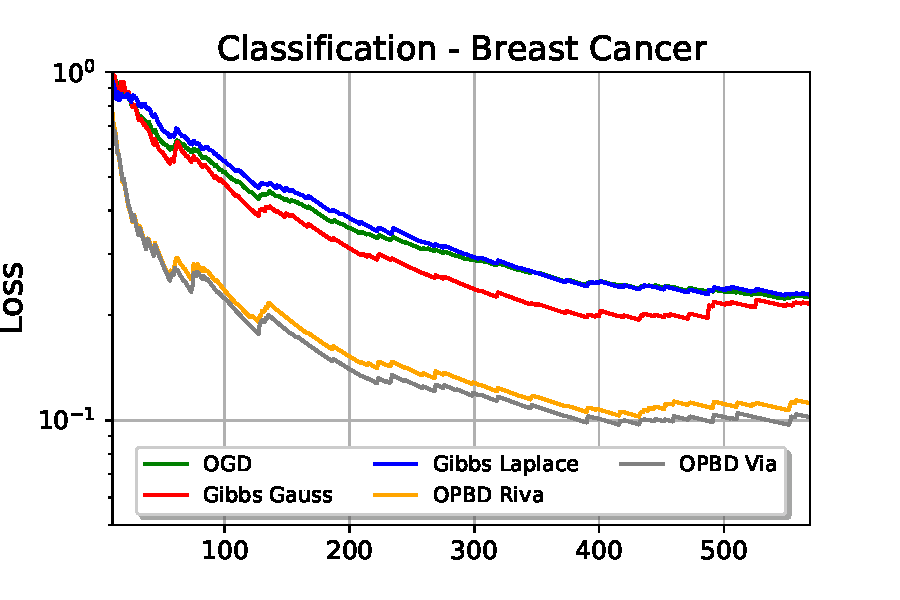
\includegraphics[width=\textwidth]{chapter_3/figures/class_breast.pdf}
  \end{subfigure}~
  \begin{subfigure}[b]{0.45\textwidth}
    \centering
    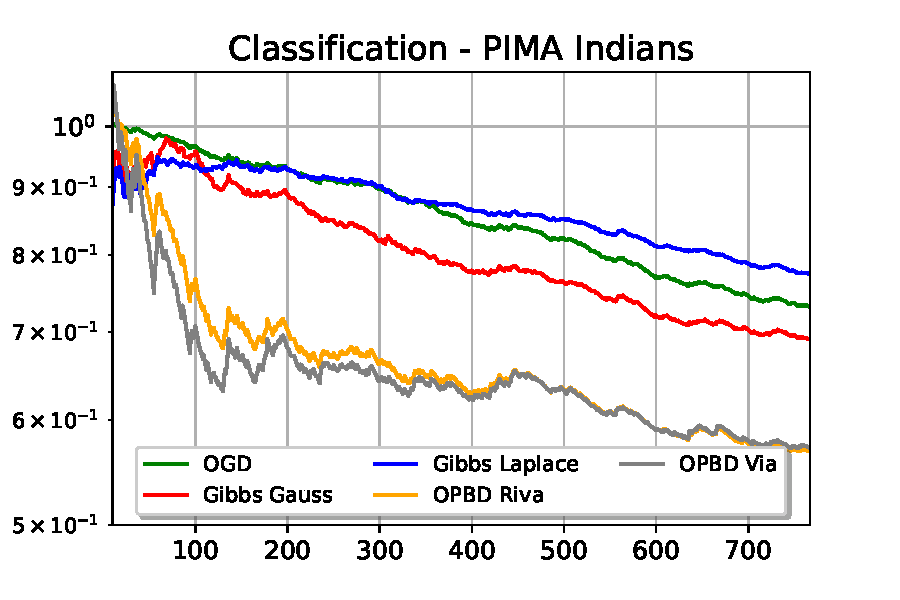
\includegraphics[width=\textwidth]{chapter_3/figures/class_diabetes}
 \end{subfigure}\\
 \begin{subfigure}[b]{0.45\textwidth}
   \centering
   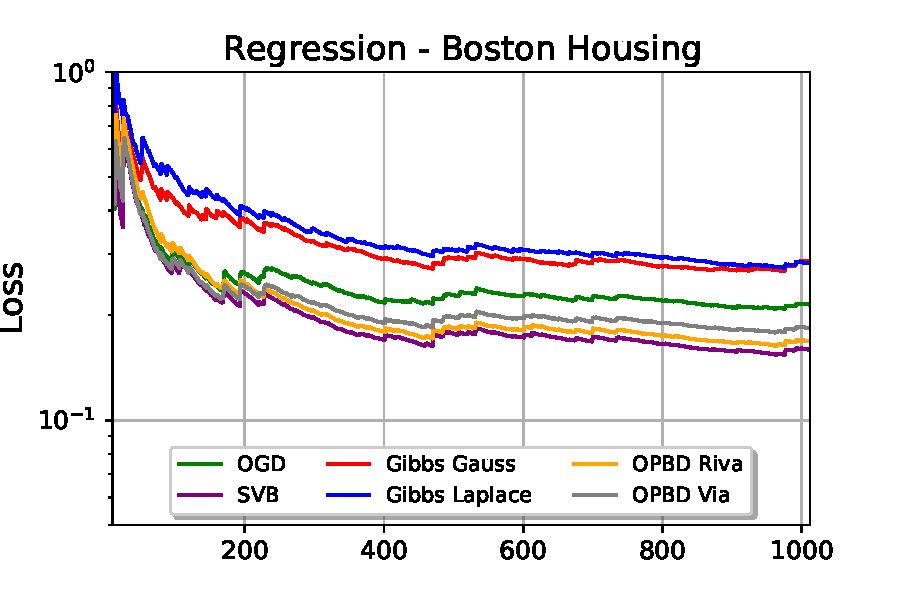
\includegraphics[width=\textwidth]{chapter_3/figures/reg_boston}
\end{subfigure}~
\begin{subfigure}[b]{0.45\textwidth}
  \centering
  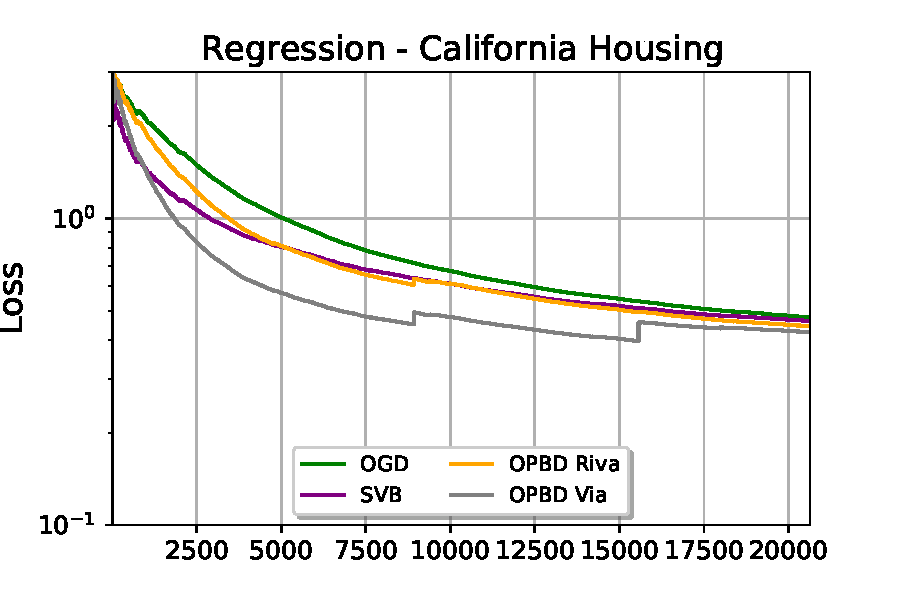
\includegraphics[width=\textwidth]{chapter_3/figures/reg_california}
\end{subfigure}
\caption{Averaged cumulative losses for all four considered datasets. 'Gibbs Gauss' denotes OPB with Gaussian Prior, 'Gibbs Laplace' denotes OPB with Laplace prior. 'OPBD Riva' denotes OPBD with $\Psi_{\normalfont1}$, 'OPBD Via' denotes OPBD with $\Psi_{\normalfont2}$. }
\label{fig: exp_results}
 \end{figure}

 \paragraph{Empirical findings.} OPB with Gaussian prior ('Gibbs Gauss') outperforms OGD on all datasets except California Housing (on which this method is not implemented ) while OPB with Laplace prior ('Gibbs Laplace') always fail w.r.t. OGD. OPB methods fail to compete with SVB on the Boston Housing dataset. OPBD methods compete with SVB on regression problems and clearly outperforms OGD on classification tasks. OPBD with $\Psi_{\normalfont2}$ (labeled as 'OPBD Via' in \Cref{fig: exp_results}) performs better on the California Housing dataset while OPBD with $\Psi_{\normalfont1}$ (labeled as 'OPBD Riva') is more efficient on the Boston Housing dataset. Both methods perform roughly equivalently on classification tasks.  This brief experimental validation shows the consistency of all our online procedures as we observe a visible decrease of the cumulative losses through time. It particularly shows that OPBD procedures improve on OGD on those dataset. We refer to \Cref{sec: error_bars} for additional table gathering the error bars of our OPBD methods.

\paragraph{Why do we perform better than OGD?} As stated in \Cref{sec: OPBD_procedure}, OGD can be recovered as a Gaussian approximation of the exponential weights algorithm (EWA). Thus, a legitimate question is why do we perform better than OGD as our OPBD methods are also based on a Gaussian surrogate of EWA?  \cite{hoeven2018many} only used Gaussians distributions with fixed variance as a technical tool when the considered predictors are the Gaussian means. In our work, we exploited a richer characteristic of our distributions in the sense our predictors are points sampled from our Gaussians and not only the means. This also has consequences in our learning algorithm as at time $i$ of our \Cref{alg: OPBD_alg}, our optimisation step involves a noise $\varepsilon_i\sim \mathcal{N}(0,\sigma^2\mathbf{I})$. Thus, we believe that OPBD methods should perform at least as well as OGD.
We write 'at least' as we think that the higher flexibility due to this additional level of randomness might result in slightly better empirical performances, as seen on the few datasets in \Cref{fig: exp_results}.





\section{Online PAC-Bayes for heavy-tailed losses.}
\label{sec: heavy-tailed}

Results of \Cref{sec: main_bound} exploited a PAC-Bayesian theorem of \citet{rivasplata2020pac} to perform, however, we note that the OL framework, by considering non-\iid data is compatible with the supermartingale toolbox of \Cref{chap: pb-ht}. We then show that it is possible to obtain anytime-valid OPB bounds for heavy-tailed losses, extending our results. Note however that such an extension can have consequences in terms of algorithmic procedures.

We now state the main theorem of this section.

\begin{theorem}[An OPB bound for heavy-tailed losses]
  \label{th: opb-ht}
  For any distribution over the dataset $\S$, any $\lambda>0$ and any online predictive sequence (used as priors) $(\P_{i})_{i\geq 1}$, we have with probability at least $1-\delta$ over the sample $\S\sim\D_{\S}$, the following, holding for the data-dependent measures $\P_{i,\S}:= \P_{i}(\S,.)$ any posterior sequence $(\Q_{i})_{i\geq 1}$ and any $m\geq 1$:

  \begin{multline*}
     \sum_{i=1}^m \mathbb{E}_{h_i\sim \Q_{i}}\left[ \mathbb{E}[\ell(h_i,\z_i) \mid \mathcal{F}_{i-1}]    \right]  \leq \sum_{i=1}^m \mathbb{E}_{h_i\sim \Q_{i}}\left[ \ell(h_i,\z_i) \right] \\+\frac{\lambda}{2}\sum_{i=1}^m \mathbb{E}_{h_i\sim \Q_{i}}\left[ \hat{V}_i(h_i,\z_i) + V_i(h_i) \right]
     + \sum_{i=1}^m\frac{\operatorname{KL}(\Q_{i}, \P_{i,\S})}{\lambda}  + \frac{\log(1/\delta)}{\lambda}.
  \end{multline*}
  With for all $i$, $\hat{V}_i(h_i,\z_i)= (\ell(h_i,\z_i)-\mathbb{E}_{i-1}[\ell(h_i,\z_i)])^2$ is the empirical variance at time $i$ and $V_i(h_i)= \mathbb{E}_{i-1}[\hat{V}(h_i,\z_i)]$ is the true conditional variance.
\end{theorem}

Proof lies in \Cref{sec: proof_main_thm_online-ht}.

\textbf{Analysis of the bound.} This bound is, to our knowledge, the first Online PAC-Bayes bound in literature holding for heavy-tailed losses. It is semi-empirical as the variance and empirical variance terms have theoretical components. However, these terms can be controlled with assumptions on conditional second-order moments and not on exponential ones (as made in \Cref{sec: main_bound} where the bounded loss assumption was used to obtain conditional subgaussianity). To emphasise our point, we consider as in \Cref{sec: iid_case} the case of the quadratic loss $\ell(h,z)= (h-z)^2$. Here, we only need to assume that our data have a finite variance if we restrict our posteriors to have both bounded means and variance. Also the meaning of the online predictive sequence $\P_{i}$ is that we must be able to design properly a sequence of priors before drawing our data, this can be for instance an online algorithm which generate a prior distribution from past data at each time step.

Finally, we note that if we assume being able to bound simultaneaously all conditional means and variance (which is strictly less restrictive than bounding the loss), then \Cref{th: opb-ht} suggests a new online learning objective which is an online counterpart to \Cref{eq: optim_obj}.

\begin{align}
    \forall i\geq1\; \hat{\Q}_{i+1}&= \underset{\Q\in\mathcal{M}(\mathcal{H})}{\mathrm{argmin}} \mathbb{E}_{h_i\sim \Q} \; \left[\ell(h_i,\z_i)+ \frac{\lambda}{2}\ell(h_i,\z_i)^2\right] + \frac{\operatorname{KL}(\Q, \P_{i,\S})}{\lambda}
\end{align}

While the algorithm differs from the one derived \Cref{th: main_thm_online}, we can still draw many links with this theorem.

\begin{itemize}
  \item If we assume our loss to be bounded, then we can upper bound our empirical/theoretical variance terms to recover exactly \Cref{th: main_thm_online}. \Cref{th: opb-ht} then shows that finite order two moments are sufficient to perform online PAC-Bayes.
  \item Another crucial point lies on the range of our result which holds with high probability for any countable posterior sequence $(\Q_{i})_{i\geq 1}$, any time $m$ and the priors $(\P_{i,\Sm})_{i\geq 1}$.
  This is far much general than \Cref{th: main_thm_online} which holds only for a single $m$ and a single posterior sequence $(\Q_{i,\Sm})_{i=1..m}$. This happens because a preliminary theorem from \citet{rivasplata2020pac} has been used instead of the change of measure inequality (\Cref{l: change_meas}). This preliminary theorem has imposed conditionnal subgaussianity to deal with the exponential moment. On the contrary, the use of the change of measure inequality alongside the supermartingale toolbox of \Cref{chap: pb-ht} allowed a result holding for any posterior sequence, and any time simultaneously.
\end{itemize}






 \section{Conclusion}

 \Cref{chap:online-pb} bridges a gap between online learning and generalisation. As seen in \Cref{sec: experiments}, considering online PAC-Bayes procedures mitigates the impact of the prior in the learning process and thus, fit the optimisation view of the prior as in initialisation point (\Cref{fig: recap-optim}), yielding performances at least comparable to online gradient descent. 
However, while Online PAC-Bayes is a promising step forward optimisation, with time-efficient procedures (\Cref{sec: disintegrated_bounds}), some questions remains: \textit{(i)} Is it possible to propagate the view of prior as initialisation directly for batch algorithms? \textit{(ii)} Is it possible to obtain PAC-Bayes learning algorithms directly for deterministic predictors instead of using disintegrated results in order to be consistent with practitioners, often avoiding stochastic predictors?

 Elements of answer to \textit{(i)} lie in \Cref{chap:gen-flat-minima}, showing that flat minimum, often attained in the context of deep neural network with much more parameters than training data, allows to attenuate the impact of the prior through a fast convergence rate. \textit{(ii)} is tackled in \Cref{chap: wass-pb,chap: wpb-practical} where the KL divergence is traded for a Wasserstein distance. 


